\textbf{2-1} 【题1】试证明如热图2-1-1所示的理想气体循环过程的比热 $c$ 必不为常量.
\begin{center}
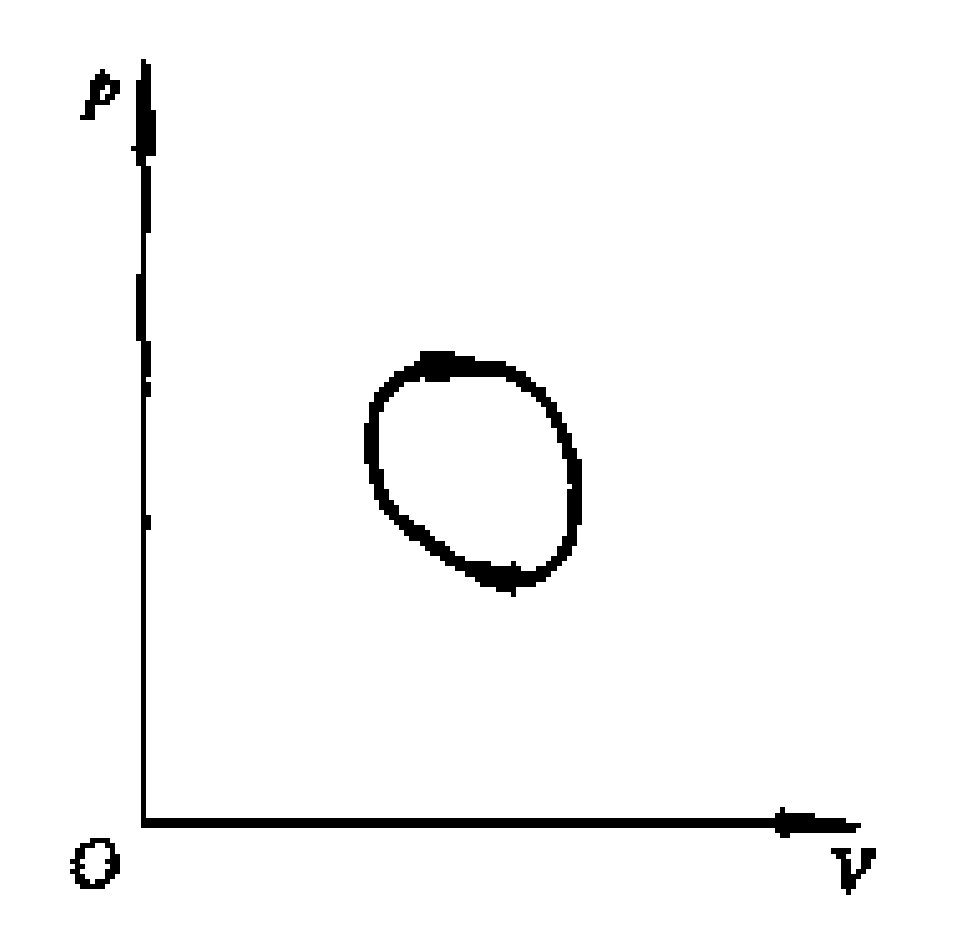
\includegraphics[width=0.2\textwidth]{figures/热图2-1-1.jpg}
\end{center}
\vfill

\textbf{2-2} 【题2】摩尔质量为 $\mu$ ，等体比热为 $c_{\mathrm{V}}(c_{\mathrm{V}}$ 为常量)的理想气体所经历的 $x$ 过程如热图2-2-1所示．若在此 $p - V$ 坐标面上，把上述 $x$ 过程向下平移 $p_0(p_0 > 0)$ ，则所得之曲线刚好是该理想气体温度为 $T_{0}$ 的等温过程．

1. 试确定 $x$ 过程中的温度下限，并指明该温度在 $x$ 过程曲线的哪个部位。

2. 试导出 $x$ 过程中比热 $c$ 与压强 $p$ 的定量关系, 并画出 $c \sim p$ 曲线.

\begin{center}
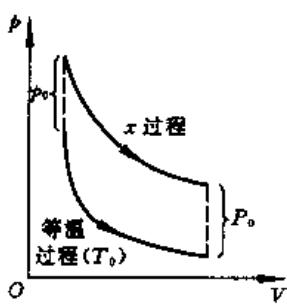
\includegraphics[width=0.2\textwidth]{figures/热图2-2-1.jpg}
\end{center}
\vfill

\newpage
\textbf{2-3} 【题3】质量为 $M$ ，摩尔质量为 $\mu$ ，等体比热为 $c_{V} = \frac{3R}{2\mu}$ 的理想气体经历的直线过程如热图2-3-1所示.

1. 试确定此过程的 $T - V$ 关系，并画图。

2. 试确定此过程中比热 $c$ 与体积 $V$ 之间的关系, 画出曲线, 并依据 $c = \frac{\mathrm{d} Q}{M \mathrm{~d} T}$ 对各段曲线 $c$ 值的正、负作定性解释.

\begin{center}
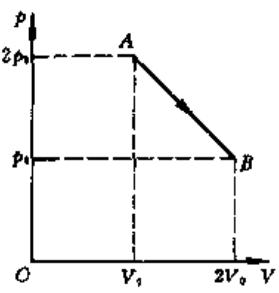
\includegraphics[width=0.2\textwidth]{figures/热图2-3-1.jpg}
\end{center}
\vfill

\textbf{2-4} 【题4】由 $\nu_{1}$ 摩尔的单原子分子理想气体与 $\nu_{2}$ 摩尔的双原子分子理想气体混合组成某种理想气体，已知该混合理想气体在常温下的绝热方程为

$$
p V ^ {\frac {1 1}{7}} = \text { 常量 }
$$

试求 $\nu_{1}$ 与 $\nu_{2}$ 的比值 $\alpha$ .
\vfill

\newpage
\textbf{9-5} 【题5】1 mol单原子分子理想气体经历某准静态过程，初态为 $(4p_0, V_0)$ ，终态为 $\left(\frac{p_0}{4}, 8V_0\right)$ . 已知在此过程的每一小过程中热功效率 $\frac{\mathrm{d}W}{\mathrm{d}Q}$ 均相同。试求此过程中气体对外界所作总功 $W$ 。
\vfill

\textbf{2-6} 【题6】2 mol单原子分子理想气体从某初态经历热容量为 $C=2R(1+0.01T)$ 的准静态过程，到达温度为初态温度2倍、体积为初态体积 $\sqrt{2}$ 倍的终态。试求内能增量 $\Delta U$ 及系统对外所作的功 W。
\vfill

\newpage
\textbf{2-7} 【题7】空气是混合气体,其中的质量分配是,氮气约占 $76.9\%$ , 氧气约占 $23.1\%$ , 其余成分可忽略不计. 现有一气缸, 缸内充有空气, 并装有一些由细钢丝做成的钢丝棉. 设气缸内的活塞能无摩擦地运动, 设缸内气压恒定为 $1 \mathrm{atm}$ . 设缸内非常缓慢地进行化学反应, 设化学反应生成 $1 \mathrm{mol}$ 的 $\mathrm{Fe}_{2} \mathrm{O}_{3}$ 后, 因氧气耗尽而中止. 已知化学反应过程是在 $1 \mathrm{atm}, 300 \mathrm{~K}$ 条件下进行的, 在此过程中系统释放出 $8.24 \times 10^{5} \mathrm{J}$ 的热量.

试求在此过程中:1. 系统内能的改变量.2. 缸内气体内能的改变量.3. 缸内氮气密度的改变量.

设缸内气体可视为理想气体．设1 mol氧气和1 mol氮气的内能均为 $\frac{5}{2}RT$ ．设缸内钢丝棉等固态物质与缸内气体相比，所占体积很小，可忽略不计．
\vfill

\textbf{2-8} 【题8】如热图2-8-1，一固定的直立气缸，它由上、下两个相互连通的圆筒构成。上部圆筒的体积为 $V_{m}$ ，其中有一个质量为 $2m$ 、面积为 $2S$ 的薄活塞A。下部圆筒足够长，其中有一个质量为 $m$ 、面积为 $S$ 的活塞B。两圆筒由一细而短的管道连通，两活塞均可在各自的圆筒内无摩擦地上下滑动，活塞A的上方盛有 $1\mathrm{mol}$ 的理想气体，活塞A、B之间盛有某种气体，活塞B下方与大气连通。开始时整个系统处于平衡态，A上方理想气体的温度为 $T_{0}$ ，已知该理想气体每摩尔的内能 $U = CT$ ，其中 $C$ 为常量， $T$ 为热力学温度，活塞B下方的大气压强为常量 $p_{0}$ ，设气缸壁、管道、活塞均不导热。然后，通过置于上部圆筒顶端的电热丝 $L$ 对活塞A上方的气体缓慢加热，设在整个加热过程中传递给A上方气体的热量为 $Q_{0}$ 。试问达到平衡时，A上方气体的温度 $T_{f}$ 是多少？
\begin{center}
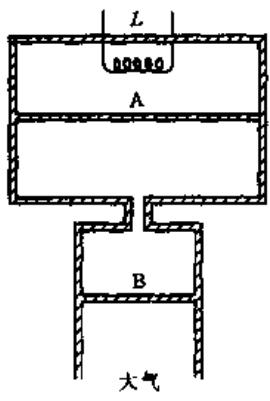
\includegraphics[width=0.15\textwidth]{figures/热图2-8-1.jpg}
\end{center}
\vfill

\newpage
\textbf{2-9} 【题9】如热图2-9-1，A和B是两个圆筒形绝热容器，中间用细的短管连通，短管中有导热性能良好的阀门 K, 短管与阀门对外绝热. F 是带柄的绝热活塞, 与容器 A 的内表面紧密接触, 不漏气, 且摩擦可忽略不计.

开始时 K 关闭, F 处于 A 的左端. A 中有 n 摩尔理想气体, 温度为 $T_{0}$ ; B 中为真空. 现在向右推动 F, 直到 A 中气体的体积与 B 的容积相等. 在此过程中, 已知对气体作功为 W, 气体温度升为 $T_{1}$ , 然后将 K 稍稍打开一点, 使 A 中的气体缓慢地向 B 扩散, 同时让活塞 F 缓慢地前进, 并保持 A 中活塞 F 附近气体的压强近似不变. 试问在此过程中, 气体最后的温度是多少? 设活塞、阀门、容器的热容量均可不计.
\begin{center}
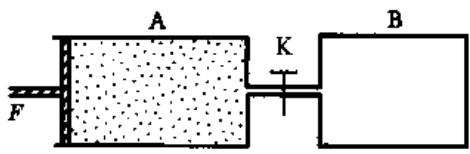
\includegraphics[width=0.3\textwidth]{figures/热图2-9-1.jpg}
\end{center}
\vfill

\textbf{2-10} 【题10】如热图2-10-1，在一以绝热壁包围的刚性圆柱形封闭气缸内，装着一个有小阀门 $L$ 的绝热活塞，在气缸的 $A$ 端还装有电热器 $\mathbf{H}$ ，可用于加热气体。

开始时, 活塞紧贴气缸 B 端的内壁, 小阀门 L 关闭. 整个气缸内装有一定质量的理想气体, 其温度为 $T_{0}$ . 然后设法把活塞推到气缸中央, 设活塞与气缸壁之间的摩擦可以忽略, 并用销钉 F 将活塞固定住, 这样气缸被分成体积相等的左、右两室, 如热图2-10-1所示. 在上述压缩气体的过程中, 设外界对气体作功 W, 气体温度上升到 T.

再开启小阀门,经过足够长时间后关闭,并拔去销钉使活塞可以自由移动．用电热器加热气体，加热完毕并经过一定时间后，测出左室气体压强增为加热前的1.5倍，右室的体积变为原来的0.75倍．试求电热器传递给气体的热量．
\begin{center}
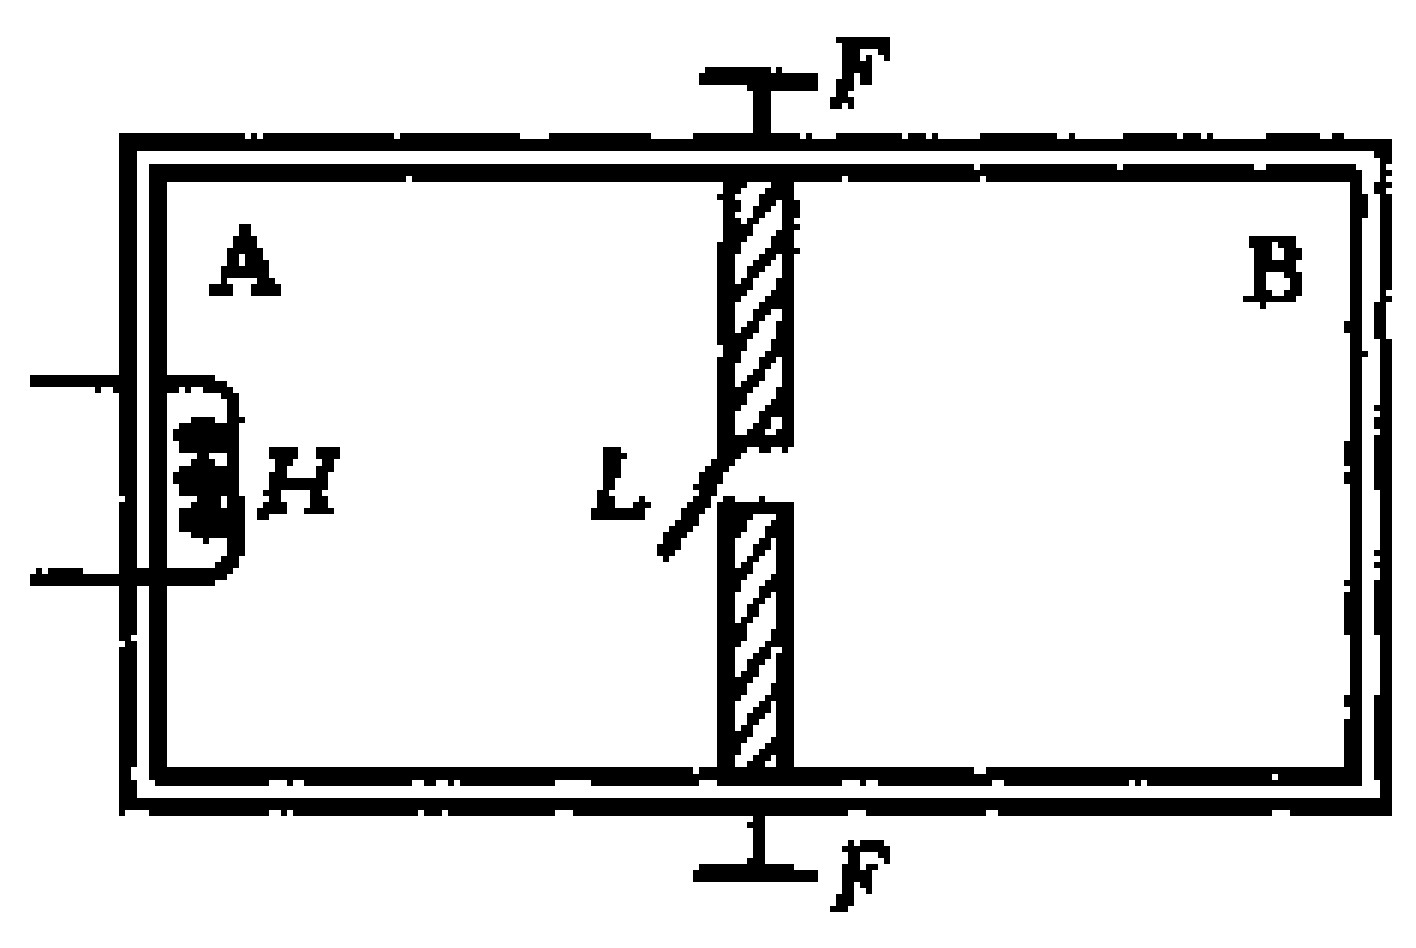
\includegraphics[width=0.2\textwidth]{figures/热图2-10-1.jpg}
\end{center}
\vfill

\newpage
\textbf{2-11} 【题11】如热图2-11-1，两个底面积均为 $S = 100\mathrm{cm}^2$ 的圆筒．左筒内气体的质量 $M_{\text{左}} = 4\mathrm{g}$ ，体积 $V_{左}=22.4L$ ，压强 $p_{左}=1\ atm$ ，温度 $T_{左}=273\ K$ 。右筒内有同种气体，质量 $M_{右}=7.44\ g$ ，体积 $V_{右}=22.4L$ ，温度 $T_{右}=273\ K$ 。左筒筒壁绝热，右筒靠大热库维持恒定的 $0\ ^{\circ}C$ 的温度。整个系统在真空中，放开左、右筒相联的活塞后，活塞移动了 $l=50\ cm$ 后达到平衡而静止。试问右筒内的气体吸收了多少热量？已知气体可视为理想气体，其定容比热为 $c_{V} = 0.75\mathrm{cal}^{*} / (\mathrm{g}\cdot \mathrm{K}) = 3.14\mathrm{J} / (\mathrm{g}\cdot \mathrm{K})$ ，设活塞与筒壁之间无摩擦。
\begin{center}
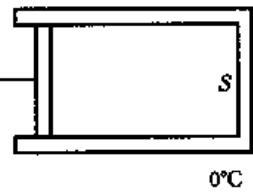
\includegraphics[width=0.2\textwidth]{figures/热图2-11-1.jpg}
\end{center}
\vfill

\textbf{2-12} 【题12】如热图2-12-1，底面积为 $100\mathrm{cm}^2$ 的圆筒，筒壁、活塞以及内部隔板都是完全绝热的。当筒内右方压强大于左方时，隔板的阀门打开。开始时有12g氮气在左方，有2g氮气在右方，左、右两方的长度均为112cm，温度均为0℃。外部压强为 $10^{5}$ Pa。氦气定体比热 $c_{V}=3.15\mathrm{J}/(\mathrm{g}\cdot\mathrm{K})$ ，定压比热为 $c_{p}=5.25\mathrm{J}/(\mathrm{g}\cdot\mathrm{K})$ 。今把活塞缓慢地推向隔板，当阀门打开时稍停片刻，尔后继续缓慢地推动活塞，直至到达隔板为止。设氮气可看作理想气体，各过程可看作准静态过程，忽略摩擦。试求所作的总功。
\begin{center}
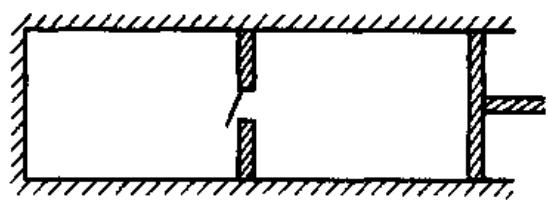
\includegraphics[width=0.25\textwidth]{figures/热图2-12-1.jpg}
\end{center}
\vfill

\newpage
\textbf{2-13} 【题13】如热图2-13-1, 长为 $2L$ 的长方形绝热容器被一个可以无摩擦地自由滑动的活塞分为容积相等的两部分 A 和 B, A 和 B 内各装有相同摩尔的单原子分子理想气体, 温度相同, 压强均为一个大气压. 今将活塞缓慢地向左推移, 当活塞移过 $\frac{1}{2}$ 时便停住, 再将活塞上的阀门打开, 使两边的气体混合. 试求容器内气体的最终压强 $p$ .
\begin{center}
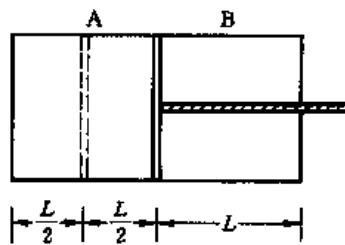
\includegraphics[width=0.2\textwidth]{figures/热图2-13-1.jpg}
\end{center}
\vfill
\newpage

\textbf{2-14} 【题14】如热图2-14-1，潮湿空气绝热地持续流过山脉．气象站 $M_0$ 和 $M_3$ 测出的大气压强都是100kPa, 气象站 $M_{2}$ 测出的大气压强为 70 kPa. 在 $M_{0}$ 处, 空气的温度是 20 ℃, 随着空气的上升, 在压强为 84.5 kPa 的高度处 (图中 $M_{1}$ ) 开始有云形成. 空气由此继续上升, 经 1500 s 之后到达山顶的 $M_{2}$ 站. 在上升过程中, 空气里的水蒸气凝结成雨落下. 设每平方米上空潮湿空气的质量为 2000 kg, 每千克潮湿空气中凝结出 2.45 g 的雨水.

1. 试求出在云层底部高度处(图中 $M_{1}$ ) 的温度 $T_{1}$ .

2. 假定空气密度随高度线性地减少, 试问云层底部 $M_{1}$ 与 $M_{0}$ 的高度差 $h_{1}$ 是多少?

3. 试问在山顶 $M_{2}$ 处测出的温度 $T_{2}$ 是多少？

4. 试求出由于空气中水蒸气的凝结, 在 3 小时内形成的降雨量. 设在 $M_{1}$ 和 $M_{2}$ 之间降雨是均匀的.

5. 试问在山脉背面的气象站 $M_{3}$ 测出的温度 $T_{3}$ 是多少？讨论 $M_{3}$ 处空气的状态，并与 $M_{0}$ 处相比较。

提示和数据:空气可看作是理想气体.水蒸气对空气热容量和密度的影响均可忽略.同样,汽化热随温度的变化也可忽略.温度的计算应精确到1K,云层底部高度的计算应精确到10m,降雨量的计算应精确到1mm.在有关的温度范围内,空气的定压比热为 $C_{p}=1005\ \mathrm{J}/(\mathrm{kg}\cdot\mathrm{K})$ .在 $M_{0}$ 处,相应于 $p_{0}$ 和 $T_{0}$ 的空气密度为 $\rho_{0}=1.189\ kg/m^{3}$ .在云层中,水的汽化热为 $L_{V}=2\ 500\ kJ/kg$ .又, $\frac{C_{p}}{C_{V}}=\gamma,\gamma=1.4,g=9.81\ m/s^{2}$ .
\begin{center}
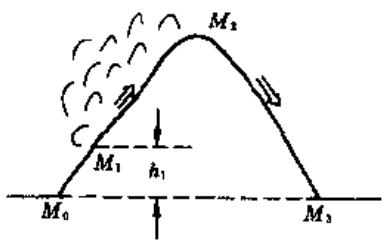
\includegraphics[width=0.25\textwidth]{figures/热图2-14-1.jpg}
\end{center}
\vfill

\newpage
\textbf{2-15} 【题15】在两端开口的竖直 $U$ 形管中注入水银，水银柱的全长为 $h$

1. 将一边管中的水银下压, 静止后撤去所加压力, 水银便会振荡起来. 试证明, 不计摩擦时, 振动周期为 $T_{1} = 2 \pi \sqrt{\frac{h}{2g}}$ .

2. 把管的右端封闭, 设被封在右管内的空气柱的高度为 $L$ , 然后使水银柱作微小的振荡, 仍设摩擦可忽略, 设空气为理想气体, 且可认为水银柱振荡时右管内被封闭的空气经历的是准静态绝热过程. 试证明, 振动周期为

$$
T _ {2} = 2 \pi \sqrt {\frac {h}{2 g + \gamma h _ {0} \frac {g}{L}}}
$$

式中 $h_{0}$ 为用水银计测量大气压的水银柱的高度, $\gamma$ 是空气的绝热指数.

3. 试证明, $\gamma = \frac{2L}{h_0}\left(\frac{T_1^2}{T_2^2} - 1\right)$ .
\vfill

\textbf{2-16} 【题16】声波可在气体管中形成驻波。现用 $1000\mathrm{Hz}$ 的声波在碘蒸气管中做实验，在温度为 $400\mathrm{K}$ 时，测得管内形成的驻波的相邻间距为 $6.77~\mathrm{cm}$ ，试问管内的碘蒸气分子是单原子的还是双原子的．已知碘的原子量是127，声波在空气中的传播速度 $v=\frac{1}{\sqrt{\rho K_{s}}}$ ，其中 $\rho$ 为气体的密度， $K_{s}$ 为气体的绝热压缩系数，定义为 $K_{s}=-\frac{1}{V}\left(\frac{dV}{dp}\right)_{绝热}$
\vfill

\newpage
\textbf{2-17} 【题17】定体摩尔热容量 $C_V$ 为常量的某理想气体。经历如热图2-17-1所示的 $pV$ 平面上的两个循环过程 $A_1B_1C_1A_1$ 和 $A_2B_2C_2A_2$ ，相应的效率分别为 $\eta_1$ 和 $\eta_2$ 。试比较 $\eta_1$ 与 $\eta_2$ 的大小（用不等式或等式表示）。
\begin{center}
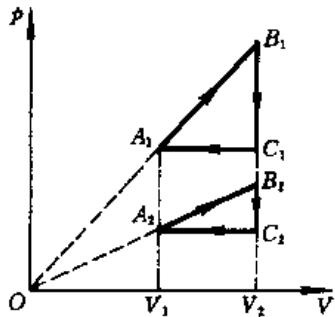
\includegraphics[width=0.2\textwidth]{figures/热图2-17-1.jpg}
\end{center}
\vfill

\textbf{2-18} 【题18】如热图2-18-1，在 $p \quad V$ 平面上用实线画出了 $C_V$ 为常量的某理想气体的几条准静态过程线，其中两条实曲线是绝热过程，三条实直线是直线过程，其延长线交于原点 $O$ 。

1. 试比较 $\eta_{12431}$ (循环过程12431的效率, 余同)与 $\eta_{12651}$ 的大小.

2. 设 $p_1^*: p_2^*: p_3^* = 1:2:3$ ，试比较 $\eta_{12431}$ 与 $\eta_{34651}$ 的大小。
\begin{center}
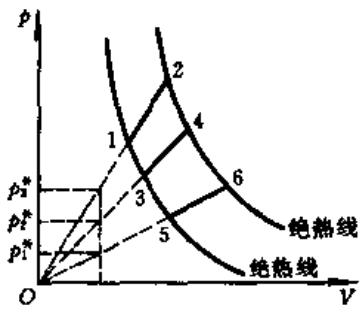
\includegraphics[width=0.2\textwidth]{figures/热图2-18-1.jpg}
\end{center}
\vfill

\newpage
\textbf{2-19} 【题19】 $1\mathrm{mol}$ 氦气(理想气体)经历如热图2-19-1所示的循环过程，热图2-19-1中AB、

BC、CA 均为直线, 有关参量已经标明. 试求循环效率 $\eta$ .

\begin{center}
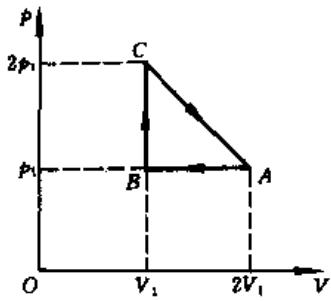
\includegraphics[width=0.2\textwidth]{figures/热图2-19-1.jpg}
\end{center}
\vfill

\textbf{2-20} 【题20】如热图2-20-1，$0.1\mathrm{mol}$ 单原子分子理想气体从初态 $(p_0 = 32.0\mathrm{Pa},V_0 = 8.00\mathrm{m}^3)$ 经 $p - V$ 图上的直线过程到达终态 $(p_{1} = 1.0\mathrm{Pa},V_{1} = 64.0\mathrm{m}^{3})$ ，再经绝热过程回到初态，试求:

1. 循环效率.

2. 上述循环的最高温度和最低温度.

\begin{center}
    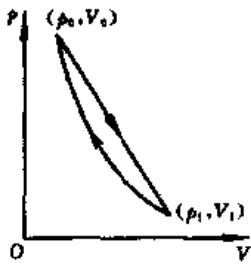
\includegraphics[width = 0.2\textwidth]{figures/热图2-20-1.jpg}
\end{center}

\vfill